\chapter{Rezultati}
\label{rez}

\section{Ekstrakcija fazora}

\textit{MATLAB} omogućava jednostavno definisanje, superponiranje i plotanje signala. Testiranje je izvršeno u pratećem m-fajlu \textit{Testiranje\_ekstrakcije.m}, a u nastavku su prikazani dobijeni rezultati.

\subsection{Djelovanje viših harmonika}

Neka je na fundamentalnu komponentu definisanu sa \ref{eq:41} superponirano prvih 5 harmonika:

\begin{equation}
    x_h(t) = 80\;sin(2wt + \pi) + 60\;sin(3wt + \frac{\pi}{6}) + 40\;sin(4wt + \frac{\pi}{2}) + 80\;sin(5wt + \frac{\pi}{12})
    \label{eq:51}
\end{equation}

Na sljedećim slikama su prikazani rezultati djelovanja navedenih 5 harmonika, zatim djelovanje tih istih harmonika sa amplitudom 10 puta većom, te djelovanje superponiranog 6. harmonika amplitude 2 i faze $\cfrac{\pi}{5}$.

\begin{figure}[H]
  \centering
  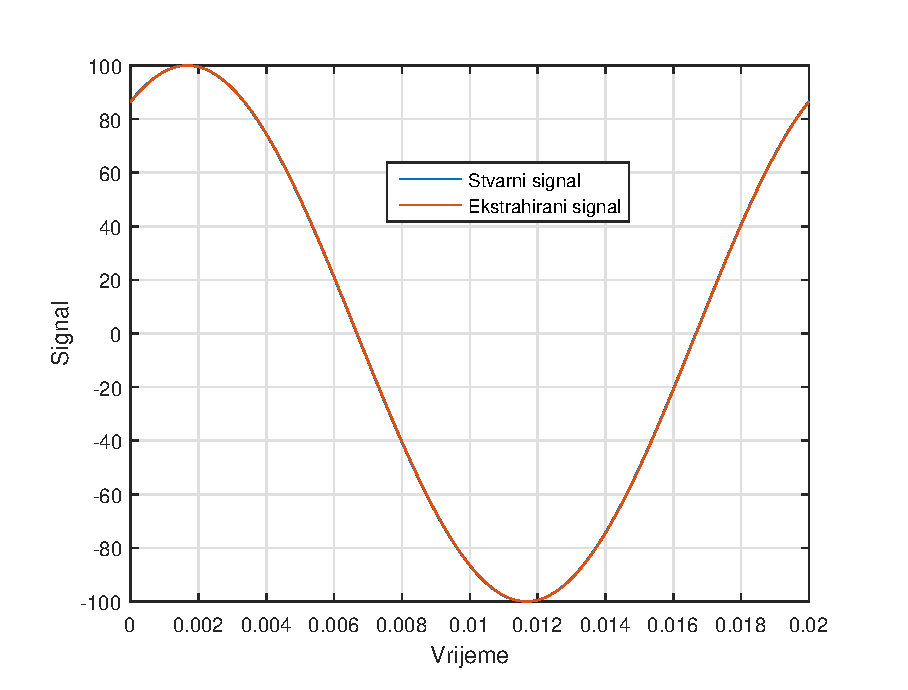
\includegraphics[width=0.7\textwidth]{Slike_rezultati/Test_h1.eps}
  \caption{Poređenje stvarnog i ekstraktovanog signala - djelovanje prvih 5 harmonika}
  \label{fig:51}
\end{figure}

\begin{figure}[H]
  \centering
  \includegraphics[width=0.7\textwidth]{Slike_rezultati/Test_h2.eps}
  \caption{Poređenje stvarnog i ekstraktovanog signala - djelovanje prvih 5 harmonika sa povećanom amplitudom}
  \label{fig:52}
\end{figure}

\begin{figure}[H]
  \centering
  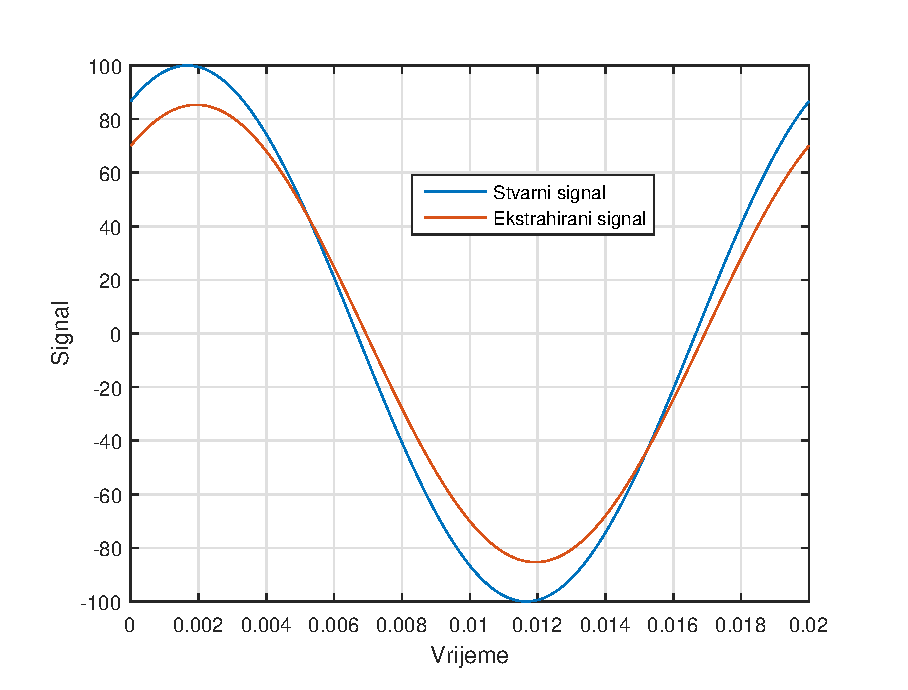
\includegraphics[width=0.7\textwidth]{Slike_rezultati/Test_h3.eps}
  \caption{Poređenje stvarnog i ekstraktovanog signala - djelovanje 6. harmonika}
  \label{fig:53}
\end{figure}

Može se zaključiti da metoda najmanjih kvadrata eliminiše djelovanje prvih 5 harmonika gotovo perfektno bez obzira na njihovu amplitudu i fazu, dok u implementiranoj LS metodi nije pretpostavljen 6. harmonik pa on uvodi grešku koja je značajna. Srećom, amplitude viših harmonika opadaju jako brzo sa porastom harmonika u praksi, a čak ako i dalje predstavljaju problem, pretpostavljanjem postajanja harmonika viših od 5. u funkciji \textit{Ekstrakcija\_signala} bi se taj problem riješio.

\subsection{Djelovanje Gaussovog bijelog šuma}

Na fundamentalnu komponentu je superponiran bijeli šum čiji se SNR (odnos signal-šum) mijenjao od -15 do 15 decibela. Za te vrijednosti SNR-a je snimljena relativna greška u amplitudi i fazi između stvarnog i ekstraktovanog signala, a to je prikazano na slici \ref{fig:54}.


\begin{figure}[H]
    \centering
    \begin{subfigure}{0.45\textwidth}
        \centering
        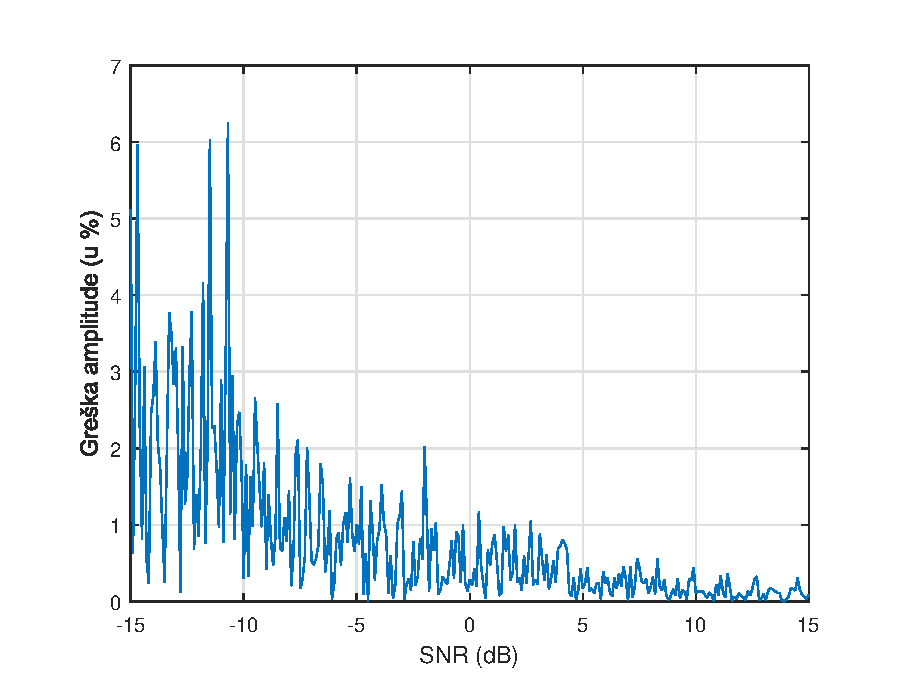
\includegraphics[width=0.9\textwidth]{Slike_rezultati/Test_bs1.eps} % first figure itself
        \caption{Greška u amplitudi (u procentima)}
    \end{subfigure}\hfill
    \begin{subfigure}{0.45\textwidth}
        \centering
        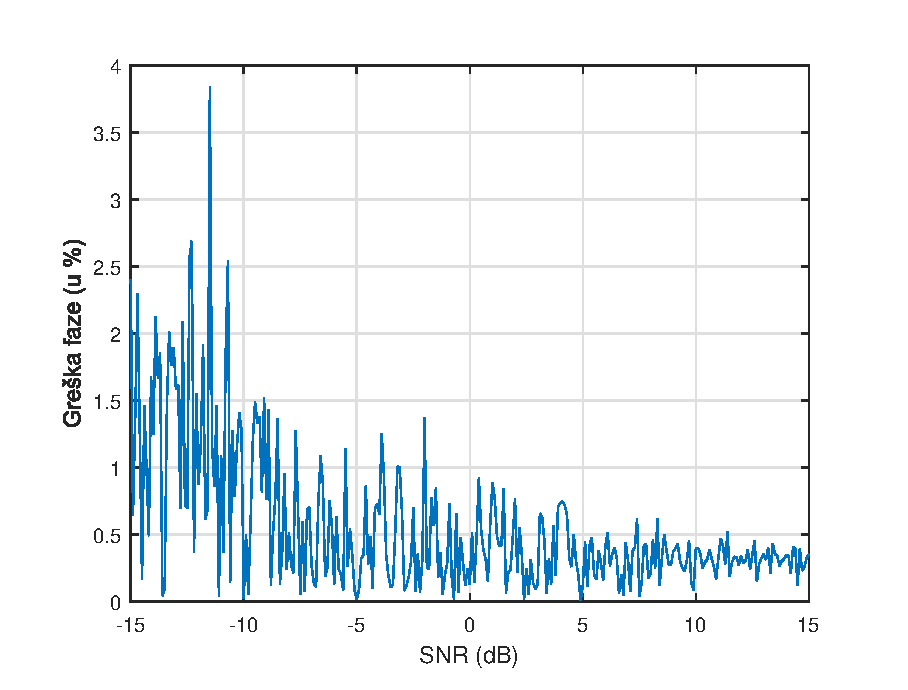
\includegraphics[width=0.9\textwidth]{Slike_rezultati/Test_bs2.eps} % second figure itself
        \caption{Greška u fazi (u procentima)}
    \end{subfigure}
    \caption{Djelovanje bijelog šuma na ekstrakciju fundamentalne komponente }
    \label{fig:54}
\end{figure}

Na posmatranom intervalu SNR-a imamo negativne vrijednosti kod kojih je šum značajno dominantniji od signala, a greške u amplitudi i fazi ne prelaze 5 do 6 procenata, dok već za vrijednosti SNR-a oko nule (signal i šum uporedive vrijednosti) greške padaju ispod 1$\%$. Za vrijednosti gdje je dominantan signal u odnosu na šum, što je obično i slučaj, greška praktično pada na nulu što je pokazatelj robusnosti metode najmanjih kvadrata na bijeli šum.

\subsection{Djelovanje DC komponente}
Kao što je navedeno i prije DC komponenta se definiše:

\begin{equation}
    x_{DC}(t) = B_0\;e^{-dt}
\end{equation}

Prvo analiziramo uticaj različitih amplituda DC komponente za fiksno $d = 10$. Na slici \ref{fig:55} su prikazane relativne greške u amplitudi i fazi prilikom ekstrakcije fundamentalne komponente na djelovanje DC komponente sa amplitudama do 10000. Vidimo da su greške u procentima ispod $1\%$ što znači da i ovu smetnju metoda najmanjih kvadrata u potpunosti eliminiše.

\begin{figure}[H]
    \centering
    \begin{subfigure}{0.45\textwidth}
        \centering
        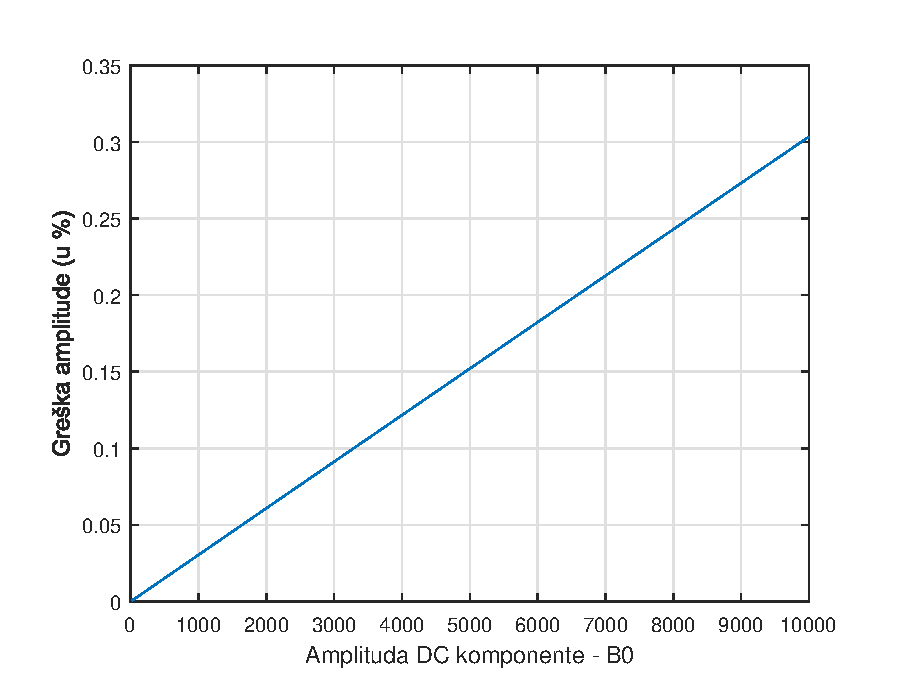
\includegraphics[width=0.9\textwidth]{Slike_rezultati/Test_dc1.eps} % first figure itself
        \caption{Greška u amplitudi (u procentima)}
    \end{subfigure}\hfill
    \begin{subfigure}{0.45\textwidth}
        \centering
        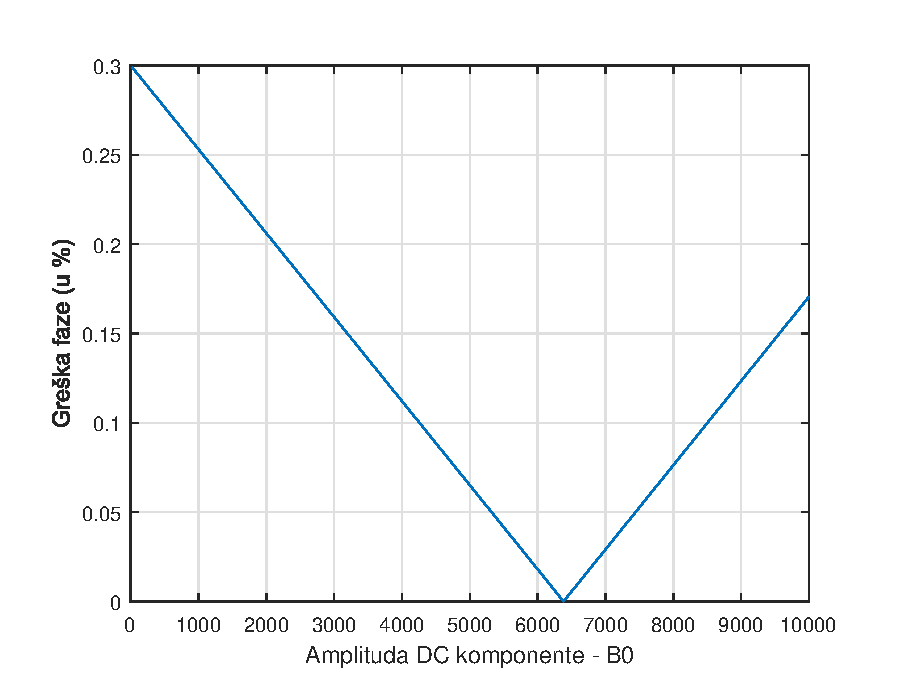
\includegraphics[width=0.9\textwidth]{Slike_rezultati/Test_dc2.eps} % second figure itself
        \caption{Greška u fazi (u procentima)}
    \end{subfigure}
    \caption{Djelovanje amplitude DC komponente na ekstrakciju fundamentalne komponente }
    \label{fig:55}
\end{figure}

Nakon analize uticaja amplituda DC komponente provodimo analizu uticaja eksponencijalnog člana DC komponente za fiksno $B_0 = 100$. Kao i za prethodne analize posmatramo relativnu grešku amplitude i faze fundamentalne komponente. Eksponencijalni član se mijenja od 0 do 10000 (\ref{fig:56}). Može se vidjeti da su procentualne greške enormne ako se pojave veoma velike vrijednosti eksponencijalnog člana što je i najveći problem ove metode. Ono što treba uzeti u obzir je da su ovdje posmatrane ekstremne vrijednosti i pitanje je da li se one pojavljuju kod distantne zaštite koja je tema ovog rada, ali je potrebno imati na umu ovaj nedostatak. 

\begin{figure}[H]
    \centering
    \begin{subfigure}{0.45\textwidth}
        \centering
        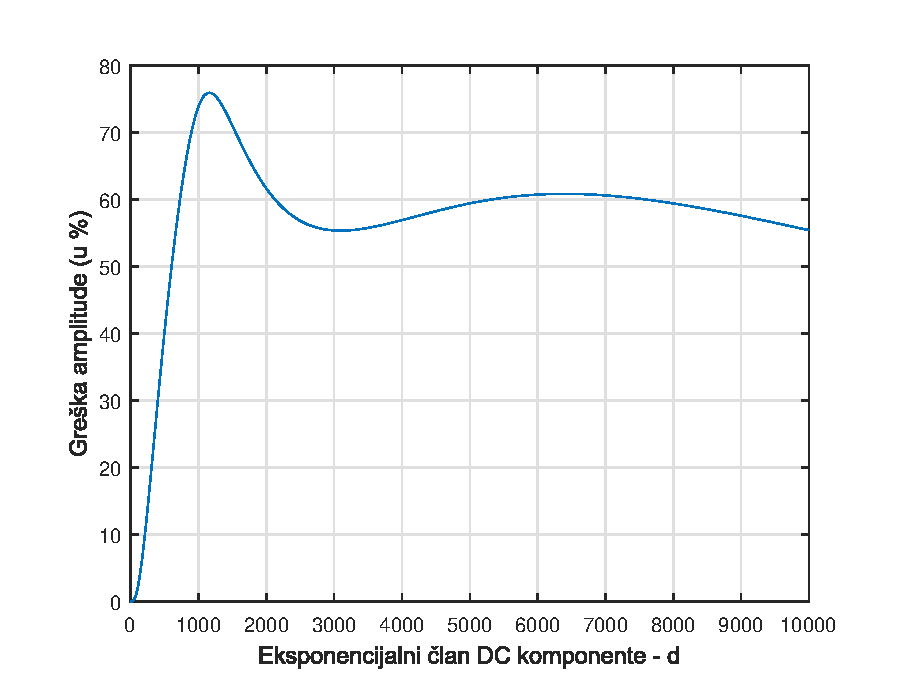
\includegraphics[width=0.9\textwidth]{Slike_rezultati/Test_dc3.eps} % first figure itself
        \caption{Greška u amplitudi (u procentima)}
    \end{subfigure}\hfill
    \begin{subfigure}{0.45\textwidth}
        \centering
        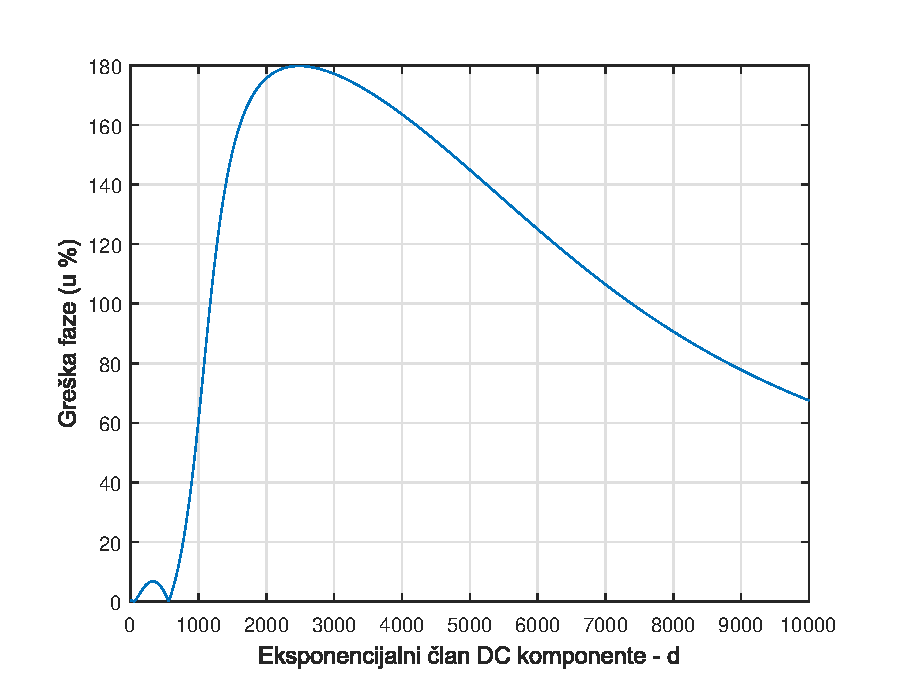
\includegraphics[width=0.9\textwidth]{Slike_rezultati/Test_dc4.eps} % second figure itself
        \caption{Greška u fazi (u procentima)}
    \end{subfigure}
    \caption{Djelovanje eksponencijalnog člana DC komponente na ekstrakciju fundamentalne komponente }
    \label{fig:56}
\end{figure}


\section{Distantna zaštita}

U prethodnom poglavlju je navedena konfiguracija simulacije, a u ovom poglavlju su priloženi rezultati koji se dobiju. Kvar je postavljen na distanci 20 km. Na osnovu položaja impedansi prije kvara tačke poligona su postavljene na sljedeći način:

\begin{itemize}
    \item $Z_1 = -450 - j450$
    \item $Z_2 = 450 - j450$
    \item $Z_3 = 450 + j450$
    \item $Z_4 = -450 + j450$
\end{itemize}

Na sljedećim slikama su prikazani GUI i položaj impedansi dobijenih mjerenjem u situaciji bez kvara, kao i prilikom trofaznog kvara, dvofaznog kvara (AC sa zemljom, BC bez zemlje) i jednofaznog kvara faze C. Može se vidjeti da je zaštita u svakom slučaju uspješno reagovala, te dala približno tačnu udaljenost (distancu). Dobijene distance za sve posmatrane kvarove su date u tabeli \ref{tab:distance}.


\renewcommand{\arraystretch}{1.5}% prosirivanje redova u tabeli
\begin{table} [!htbp]
  \caption{Izrazi za impedanse pojedinih kratkih spojeva}
  \begin{center}
  \begin{tabular}{ | c | c | c | }
	\hline
      \textbf{Vrsta kvara} & \textbf{Faze koje su sudjelovale} & \textbf{Dobijena distanca [km]} \\
    \hline 
    \hline 
     jednofazni KS sa zemljom & A &  $19.997$ \\[10pt]
    \hline
    jednofazni KS sa zemljom & B &  $19.8872$ \\[10pt]
    \hline
    jednofazni KS sa zemljom & C &  $19.8767$ \\[10pt]
    \hline
    dvofazni KS bez zemlje & A i B &  $19.9749$ \\[10pt]
    \hline
    dvofazni KS sa zemljom & A i B &  $19.9781$ \\[10pt]
    \hline
    dvofazni KS bez zemlje & B i C &  $19.799$ \\[10pt]
    \hline
    dvofazni KS sa zemljom & B i C &  $19.8035$ \\[10pt]
    \hline
     dvofazni KS bez zemlje & C i A &  $19.9081$ \\[10pt]
    \hline
     dvofazni KS sa zemljom & C i A &  $19.981$ \\[10pt]
    \hline
    trofazni KS bez zemlje & A, B i C &  $19.8795$ \\[10pt]
    \hline
     trofazni KS sa zemljom & A, B i C &  $19.8795$ \\[10pt]
    \hline
  \end{tabular}
  \label{tab:distance}    
\end{center} 
\end{table}
\renewcommand{\arraystretch}{1} % vraćeno na staro

Kao što je prethodno napomenuto, distance su izračunate sa jako velikom tačnošću što govori o kvaliteti distantne zaštite. Lokacija kvara je uspješno određena što je jedna od osnovnih funkcija distantnog releja.

\begin{figure}[H]
  \centering
  \includegraphics[width=0.9\textwidth]{Rezultati1/GUI_bezKvara.JPG}
  \caption{Korisnički interfejs GUI za slučaj bez kvara}
  \label{fig:57}
\end{figure}


\begin{figure}[H]
  \centering
  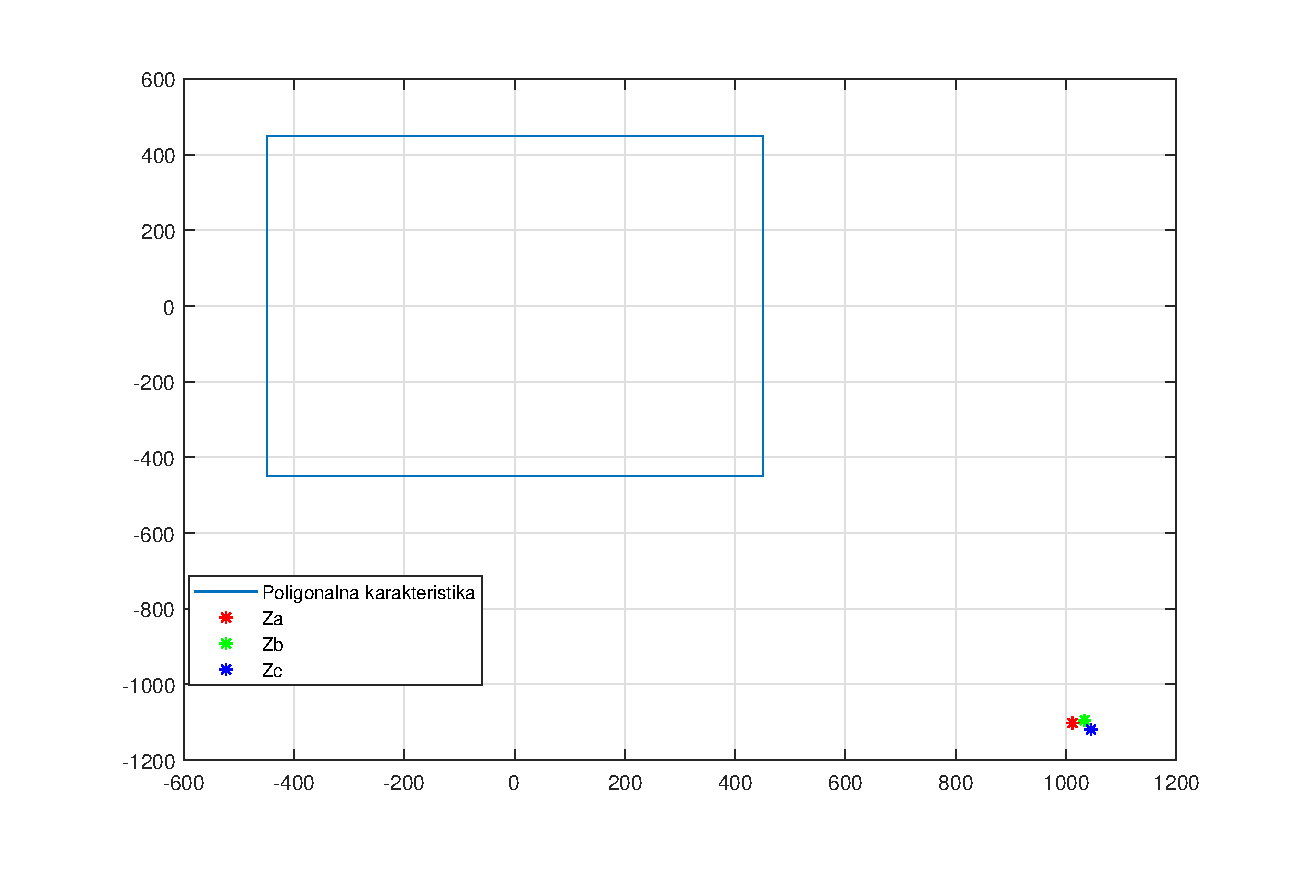
\includegraphics[width=0.8\textwidth]{Rezultati1/karakteristika_bezKvara.eps}
  \caption{Položaj impedansi u poligonalnoj karakteristici za slučaj bez kvara}
  \label{fig:58}
\end{figure}



\begin{figure}[H]
  \centering
  \includegraphics[width=0.9\textwidth]{Rezultati1/gui_3F_ABC_G.jpg}
  \caption{Korisnički interfejs GUI za trofazni KS faza ABC(sa/bez zemlje)}
  \label{fig:59}
\end{figure}


\begin{figure}[H]
  \centering
  \includegraphics[width=0.8\textwidth]{Rezultati1/karakteristika_3F_ABC_G.eps}
  \caption{Položaj impedansi u poligonalnoj karakteristici za trofazni KS faza ABC(sa/bez zemlje)}
  \label{fig:60}
\end{figure}

\begin{figure}[H]
  \centering
  \includegraphics[width=0.9\textwidth]{Rezultati1/gui_2F_AC_G.jpg}
  \caption{Korisnički interfejs GUI za dvofazni KS faza AC sa zemljom}
  \label{fig:61}
\end{figure}


\begin{figure}[H]
  \centering
  \includegraphics[width=0.8\textwidth]{Rezultati1/karakteristika_2F_AC_G.eps}
  \caption{Položaj impedansi u poligonalnoj karakteristici za dvofazni KS faza AC sa zemljom}
  \label{fig:62}
\end{figure}


\begin{figure}[H]
  \centering
  \includegraphics[width=0.9\textwidth]{Rezultati1/gui_2F_AB.jpg}
  \caption{Korisnički interfejs GUI za dvofazni KS faza AB bez zemlje}
  \label{fig:63}
\end{figure}


\begin{figure}[H]
  \centering
  \includegraphics[width=0.8\textwidth]{Rezultati1/karakteristika_2F_AB.eps}
  \caption{Položaj impedansi u poligonalnoj karakteristici za dvofazni KS faza AB bez zemlje }
  \label{fig:64}
\end{figure}

\begin{figure}[H]
  \centering
  \includegraphics[width=0.9\textwidth]{Rezultati1/gui_1F_C_G.jpg}
  \caption{Korisnički interfejs GUI za jednofazni KS faze C}
  \label{fig:65}
\end{figure}


\begin{figure}[H]
  \centering
  \includegraphics[width=0.8\textwidth]{Rezultati1/karakteristika_1F_C_G.eps}
  \caption{Položaj impedansi u poligonalnoj karakteristici za jednofazni KS faze C }
  \label{fig:66}
\end{figure}

